%=================================================================
\section{Introduction}\label{sec-intro}
\subsection{Problem Statement}
The competation \textit{Google QUEST Q\&A Labeling} is designed to 
improving automated understanding of complex question answer content.
The challenge is to use this new dataset to build predictive algorithms for different subjective aspects of question-answering. 
The question-answer pairs were gathered from nearly 70 different websites, in a "common-sense" fashion.
\begin{figure}[htbp]
    \centering
    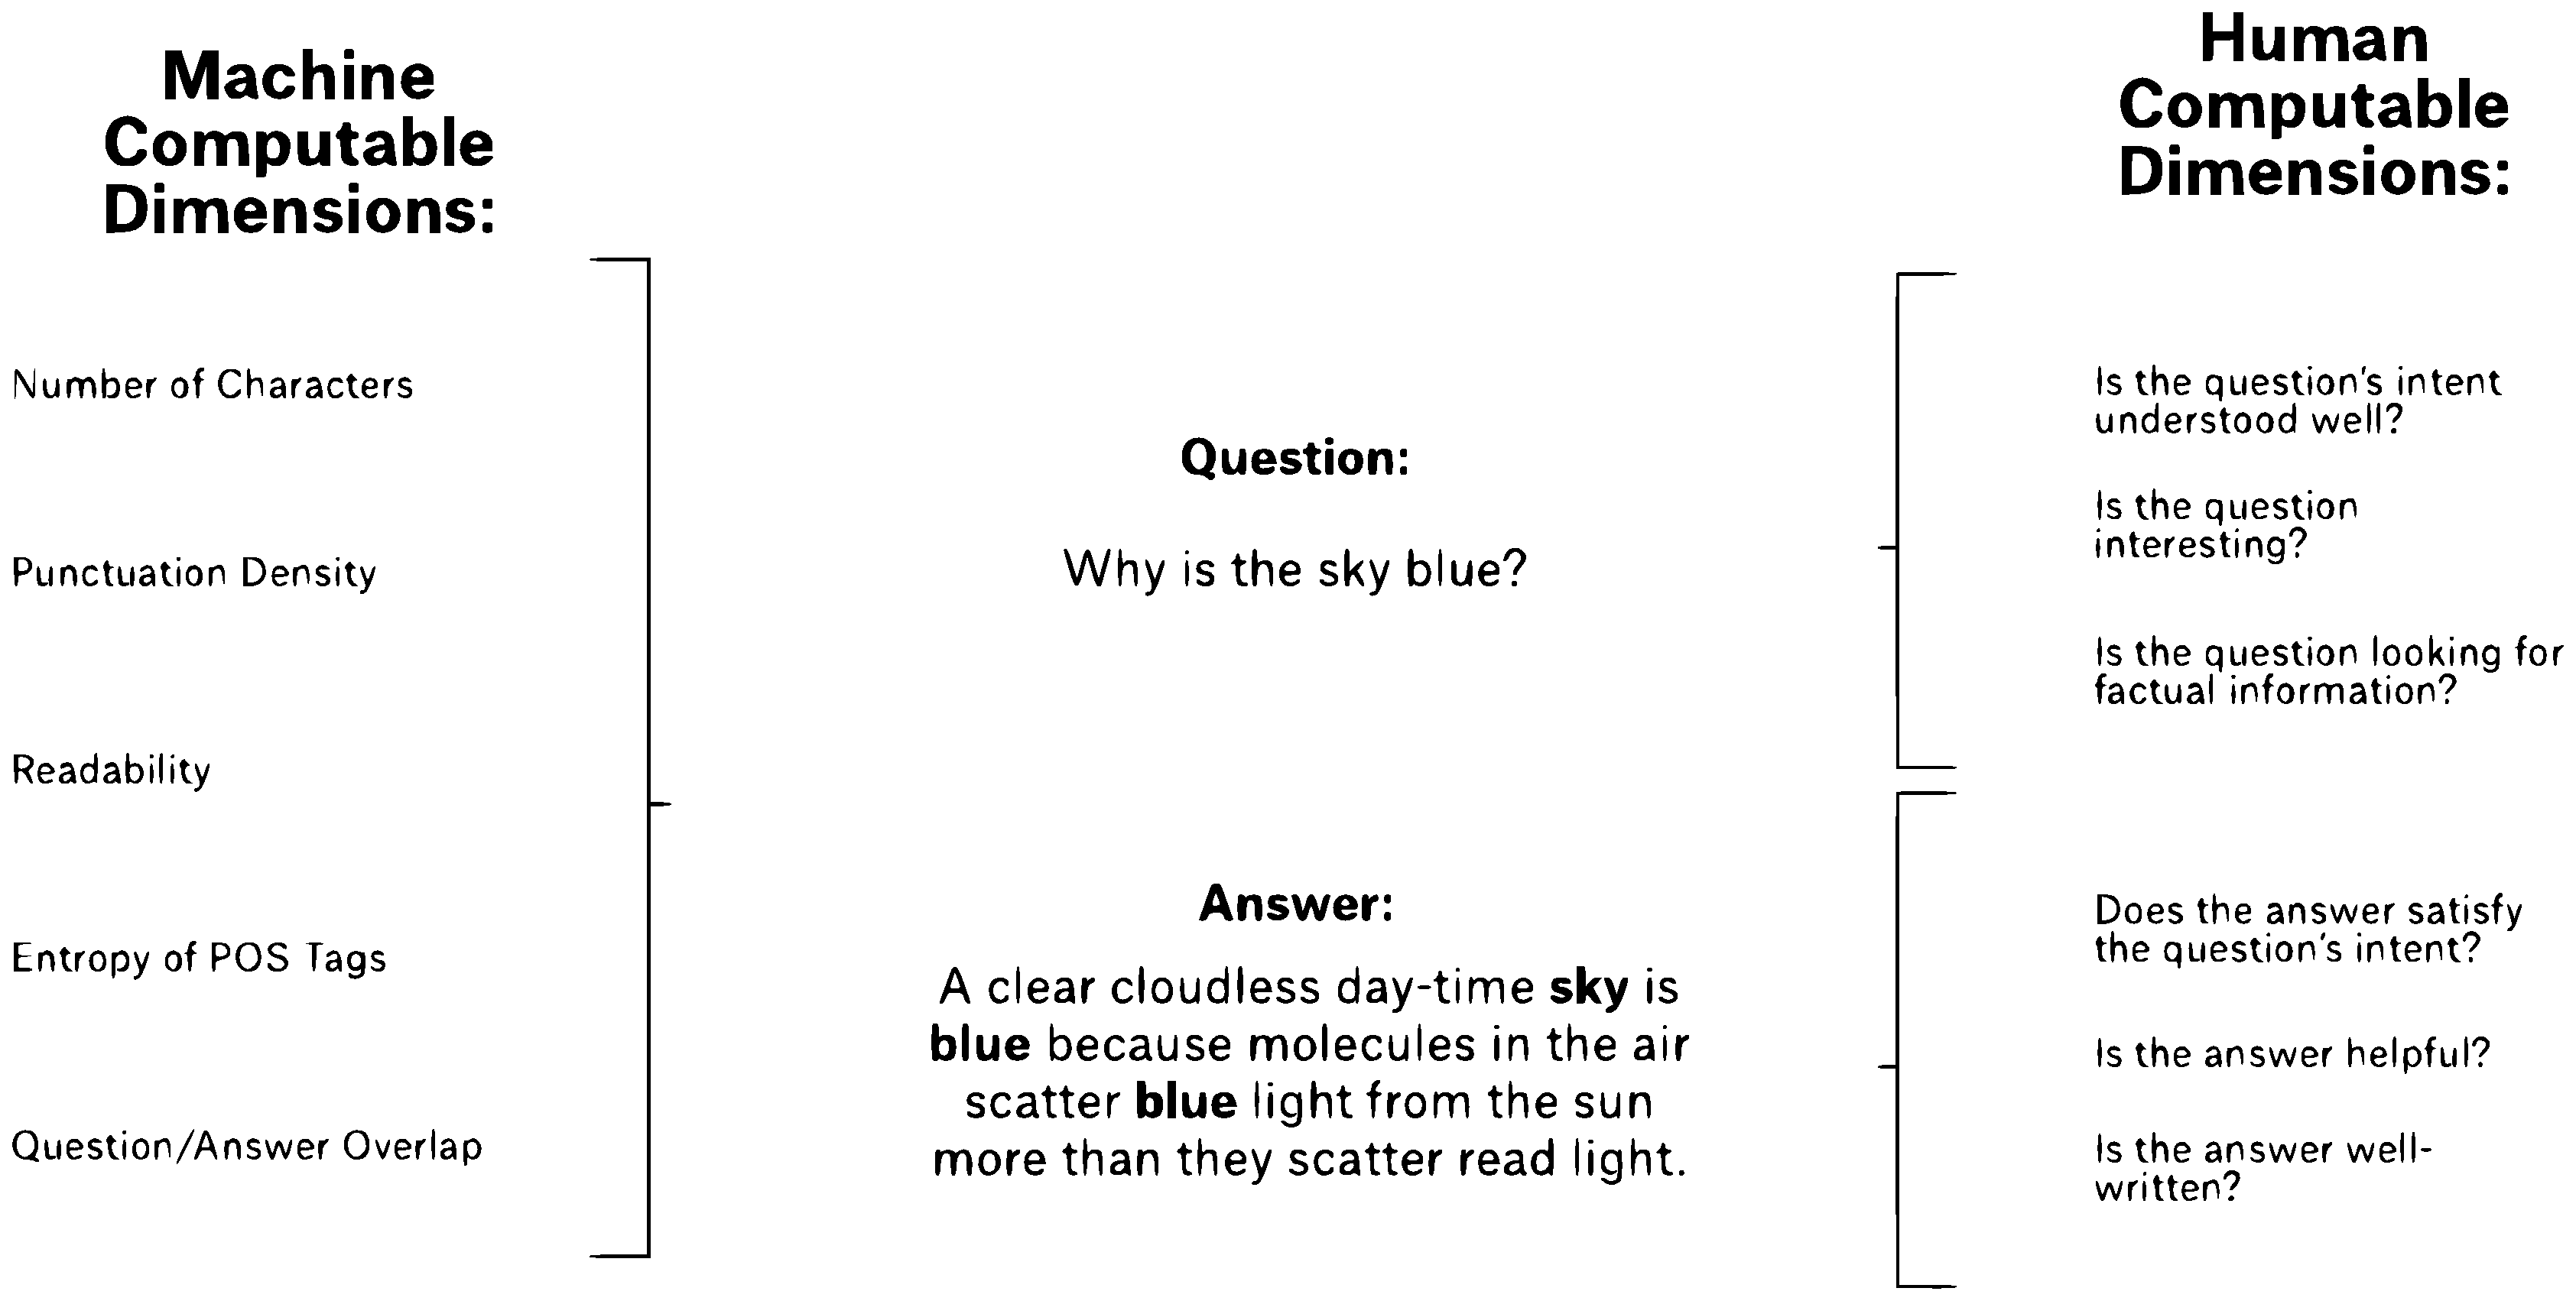
\includegraphics[width=30em]{figures/title.eps}
    \caption{Different between machine and human answer}
    \label{fig:title}
\end{figure}
\subsection{Dataset}
The dataset contains 6049 records in training set and 476 records in test set, with the following features:
\begin{itemize}
    \item Question title\&body
    \item Answer
    \item Host
    \item Category
    \item Question user
    \item Answer user
    \item Url
\end{itemize}
The targets are both continuous values in the range of $[0,1]$, representing the score of this record in the corrsponding dimension.
It contains 21 question related targets and 9 answer related targets.

\subsection{Solution}
Transformer Models such as \textit{Bert} are proven have great performance on many nlp tasks, especially for Question\&Anwser tasks.
In this competation, I will use Bert Model to solve the problem.
\section{EDA and Feature Engineering} \label{sec-eda}

\section{Method} \label{sec-method}

\section{Experiment and Analysis} \label{sec-experiment}

\section{Conclusions} \label{sec-conclusions}


The authors would like to thank \ldots

